\documentclass{article}
\usepackage{ismir,amsmath,cite}
\usepackage{graphicx}
\usepackage{color}
\usepackage{subcaption}

\title{Extracting Ground-Truth Information from MIDI Files}

%\oneauthor
% {Colin Raffel and Daniel P. W. Ellis}
% {LabROSA \\ Department of Electrical Engineering \\ Columbia University \\ New York, NY}

\threeauthors
  {First Author} {Affiliation1 \\ {\tt author1@ismir.edu}}
  {Second Author} {\bf Retain these fake authors in\\\bf submission to preserve the formatting}
  {Third Author} {Affiliation3 \\ {\tt author3@ismir.edu}}

%% To make customize author list in Creative Common license, uncomment and customize the next line
%  \def\authorname{Colin Raffel, Daniel P. W. Ellis} 

\sloppy

\begin{document}

\maketitle

\begin{abstract}
MIDI files abound and provide a bounty of information for music informatics.
We enumerate the types of information available in MIDI files and describe the steps necessary for utilizing them.
We also quantify the reliability of this data by comparing it to human-annotated ground truth.
The results suggest that further research in audio-to-MIDI alignment will facilitate the use of MIDI-derived ground-truth information for audio content-based MIR.
\end{abstract}

\section{MIDI Files}\label{sec:introduction}

MIDI (Music Instrument Digital Interface) is a hardware and software standard for communicating musical events.
First proposed in 1983 \cite{international1983midi}, MIDI remains a highly pervasive standard both for storing musical scores and communicating information between digital music devices.
Its use is perhaps in spite of its crudeness, which has been lamented since MIDI's early days \cite{moore1988dysfunctions}; most control values are quantized as 7-bit integers and information is transmitted at the relatively slow (by today's standards) 31,250 bits per second.
Nevertheless, its efficiency and well-designed specification make it a convenient way of formatting digital music information.

In the present work, we will focus on MIDI files, which in a simplistic view can be considered a compact way of storing a musical score.
MIDI files are specified by an extension to the MIDI standard \cite{international1988standard} and consist of a sequence of MIDI messages organized in a specific format.
A typical MIDI file contains timing and meter information in addition of a collection of one or more ``tracks'', each of which contains a sequence of notes and control messages.
The General MIDI standard further specifies a collection of 128 instrument types on which the notes can be played, which standardizes the playback of MIDI files and has therefore been widely adopted.

When paired with a General MIDI synthesizer, MIDI files have been used as a sort of (highly lossy) perceptual audio codec, with entire songs only requiring a few kilobytes of storage.
The early availability of this ``coding method'', combined with the expense of digital storage in the 90s, made MIDI files a highly pervasive method of storing and playing back songs before the advent of the MP3.
Even after high-quality perceptual audio codecs were developed and storage prices plummeted, MIDI files remained in use in resource-scarce settings such as karaoke machines and cell phone ringtones.
As a result, there is an abundance of MIDI file transcriptions of music available today; through a large-scale web scrape, we obtained 176,141 MIDI files with unique MD5 checksums.

Given their wide availability, we believe that MIDI files are underutilized in the Music Information Retrieval community.
In this paper, we start by outlining the various sources of information present in MIDI files and reference relevant works which utilize them in Section \ref{sec:information}.
In Section \ref{sec:utilizing}, we discuss the steps needed to leverage MIDI-derived information as ground truth for content-based MIR.
Based on these steps, we establish a baseline for the reliability of MIDI-derived ground truth by comparing it to handmade annotations in Section \ref{sec:measuring}.
Finally, in Section \ref{sec:discussion}, we argue that improving the process of extracting information from MIDI files is a viable path for creating large amounts of ground truth data for MIR.

\section{Information Available in MIDI Files}
\label{sec:information}

While various aspects of MIDI files have been used in MIR research, to our knowledge there has been no unified overview of the information they provide, nor a discussion of the availability and reliability of this information in MIDI transcriptions found ``in the wild''.
We therefore present an enumeration of the different information sources in a typical MIDI file and discuss their applicability to different MIR tasks.
Because not all MIDI files are created equal, we also computed statistics about the presence and quantity of each information source across our collection of 176,141 unique MIDI files; the results can be seen in Figure \ref{fig:statistics} and will be discussed in the following sections.

\begin{figure*}
    \centering
    \begin{subfigure}{.23\textwidth}
        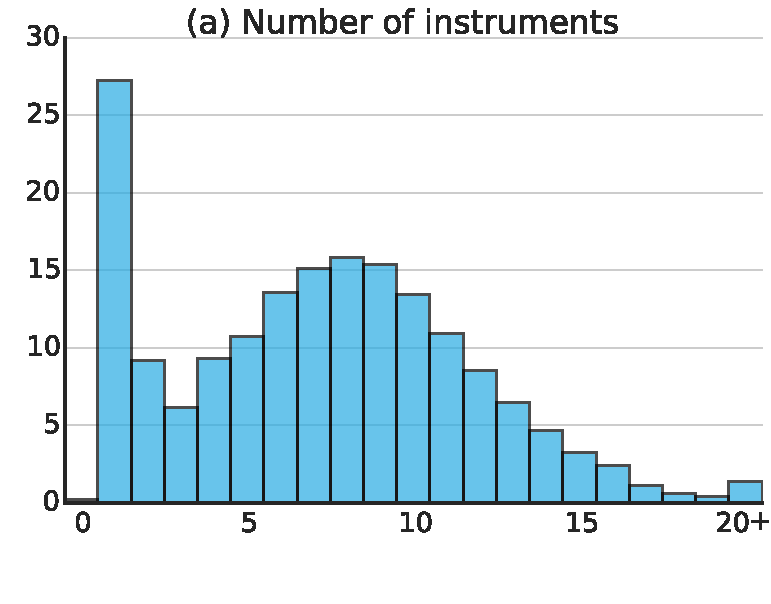
\includegraphics[width=\textwidth]{n_instruments.pdf}
    \end{subfigure}
    \begin{subfigure}{.23\textwidth}
        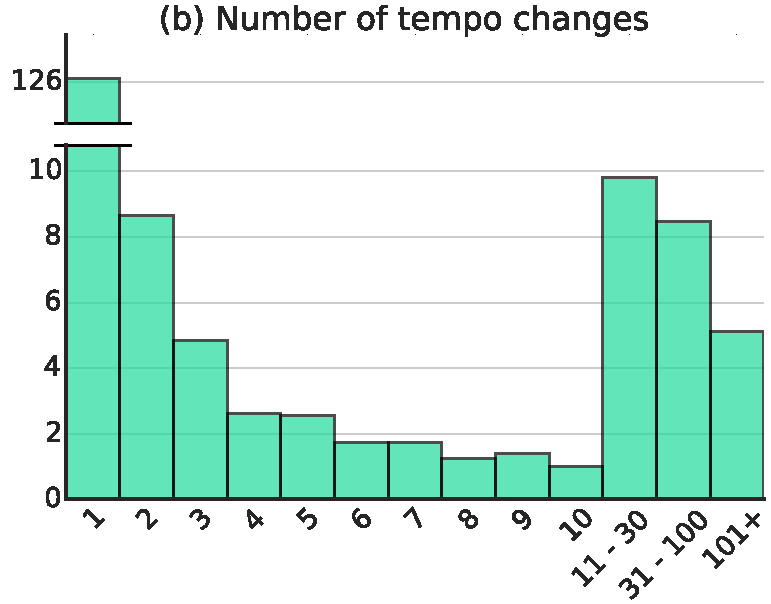
\includegraphics[width=\textwidth]{n_tempos.pdf}
    \end{subfigure}
    \begin{subfigure}{.23\textwidth}
        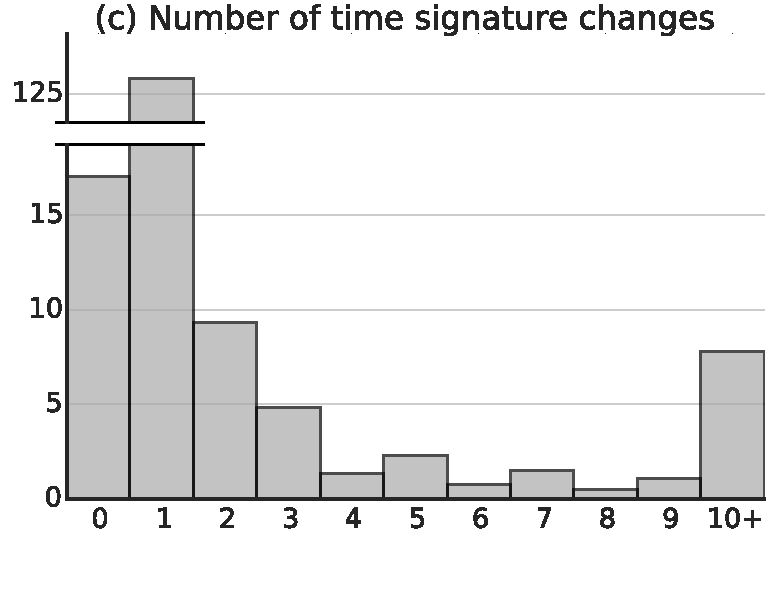
\includegraphics[width=\textwidth]{n_signatures.pdf}
    \end{subfigure}
    \begin{subfigure}{.23\textwidth}
        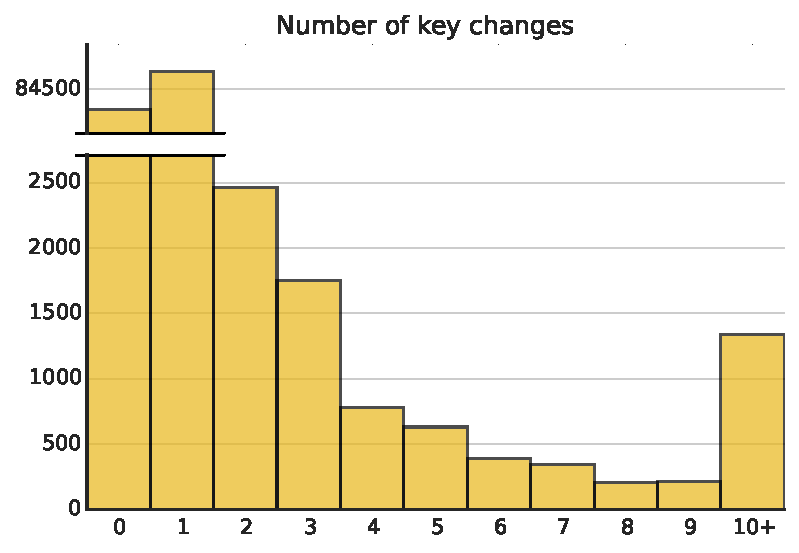
\includegraphics[width=\textwidth]{n_keys.pdf}
    \end{subfigure}

    \begin{subfigure}{.23\textwidth}
        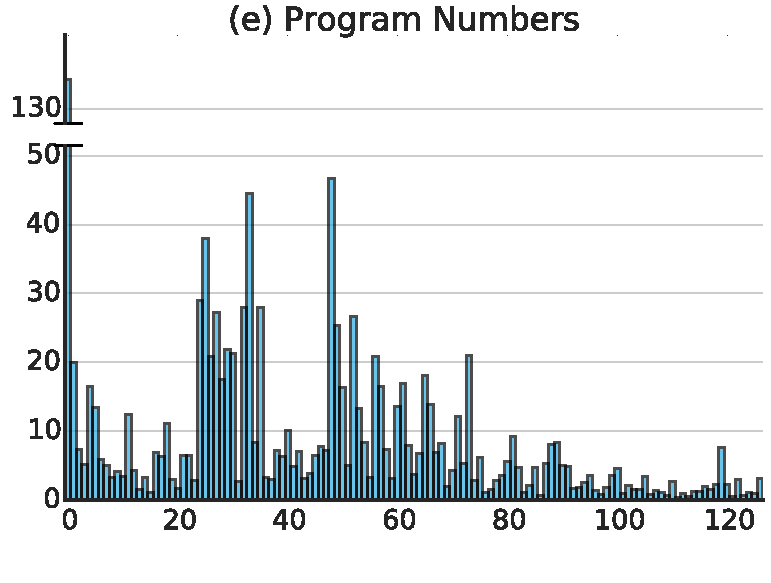
\includegraphics[width=\textwidth]{program_numbers.pdf}
    \end{subfigure}
    \begin{subfigure}{.23\textwidth}
        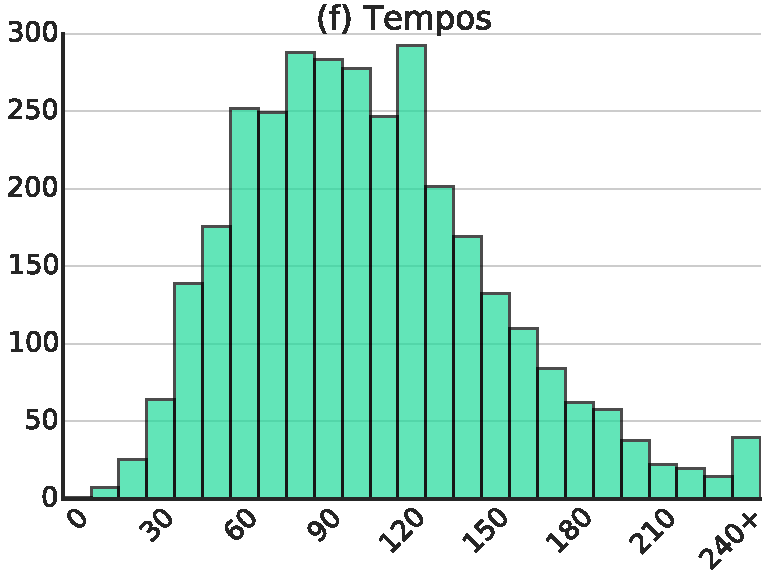
\includegraphics[width=\textwidth]{tempos.pdf}
    \end{subfigure}
    \begin{subfigure}{.23\textwidth}
        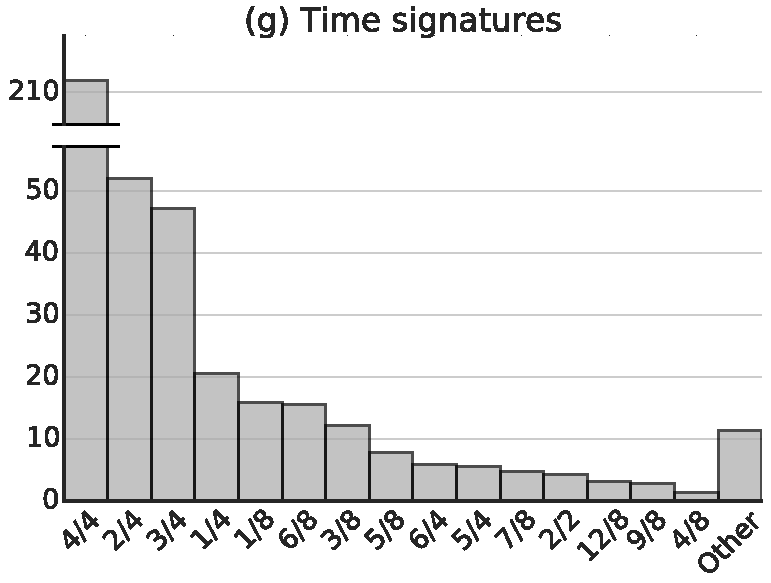
\includegraphics[width=\textwidth]{time_signatures.pdf}
    \end{subfigure}
    \begin{subfigure}{.23\textwidth}
        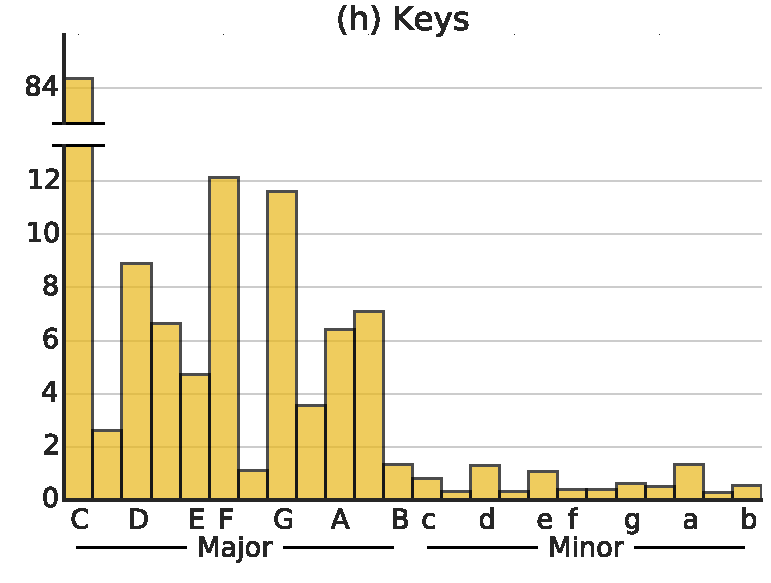
\includegraphics[width=\textwidth]{keys.pdf}
    \end{subfigure}
    \caption{Statistics about sources of information in 176,141 unique MIDI files scraped from the internet.
    Histograms in the top row show the number of MIDI files which had a given number of events for different event types; in the bottom row, we show distributions of the different values set by these events across all MIDI files.
    For example, about 125,000 MIDI files had a single time signature change event, and about 210,000 of the time signatures found in all of our MIDI files were 4/4.}
    \label{fig:statistics}
\end{figure*}

\subsection{Transcription}

For transcription and score-informed source separation

Better chroma for chord

Instrument activation

\subsection{Onsets}

Thanks to transcription.  However, of limited utility.

\subsection{Musicological Features}

Reference jSymbolic, music21

\subsection{Meter}

Beats and downbeats via time signature and tempo change events

\subsection{Key}

Key change events

\subsection{What's Missing}

Explicit labeling of melody or voice instrument

Chords, segmentation

Metadata

\section{Utilizing MIDI Files as Ground Truth}
\label{sec:utilizing}

\subsection{Matching}

Required for nearly everything.

For small collections, you might not have to do anything.

For large collections, you need sophisticated methods because of lack of metadata.

Beneficial for MIDI analysis too, thanks to matching it with audio metadata collections.

\subsection{Aligning}

Required for all time-sensitive information.

\subsection{Evaluating Quality}

In some cases, the transcription may be bad.

\subsection{Extracting Information}

Short description of \texttt{pretty\_midi}.

\section{Measuring a Baseline of Reliability for MIDI-Derived Ground Truth}
\label{sec:measuring}

Match and align to Isophonics Beatles collection

\subsection{Beat Experiment}

\subsection{Key Experiment}

\section{Discussion}
\label{sec:discussion}

As-is, a lot of the information is usable.

Improving audio-to-MIDI alignment as a proxy for getting additional metadata.

Many additional avenues for improvement of measuring quality.

\bibliography{refs}

\end{document}
